\subsection{KNN}
\subsubsection{Implementation}

The KNN algorithm is based on the fact that similar objects are close to each other. The distance between two images
denotes the similarity between them. If two images have overlapping features, from the Euclidean distance formula 
(\ref{eq:euclidean}), those features will cancel each other out and the final distance will be small.

\begin{equation}
    d = \sqrt{\sum_{i=1}^{n} (x_i - y_i)^2}
    \label{eq:euclidean}
\end{equation}

The actual implementation of the Euclidean distance in the code does not use the square root. This is because the square root
is a relatively expensive function to implement. Also the square root is a monotonic function. This means that the order of the
distances is preserved.

An other optimization of the current implementation is that the final distances array is not sorted. The
K nearest neighbors are acquired by finding the minimum value of the distances array. The time complexity of this algorithm is
O(kn) instead of O(nlogn).

The K factor is the number of neighbors that the algorithm will use to classify the image. The values of K that were used for 
testing in this implementation are 1 and 3. In general we want to use an odd number for K. This is because if we use an even
number for K we might end up with a tie. Finally, the MNIST dataset has overlapping classes. This means that the classes are
not linearly separable. For this reason larger numbers for K lead to very low accuracy.

\subsubsection{Results}

The KNN accuracy table (\ref{tab:knn}), shows the accuracy and the execution time of the KNN algorithm for different values of K.
The accuracy is the percentage of the correctly classified images. The execution time is the time it took to classify all the
images in the test dataset. The execution time is measured in seconds. 16 threads were used for the parallelization of the algorithm.

\renewcommand{\arraystretch}{1.5}

\begin{center}
\begin{table}[h]
    \centering
    \begin{tabular}{|c|c|c|c|c|}
        \hline
        K & 1 & 3 & 5 & 7 \\
        \hline
        Accuracy (\%) & 96.91 & 97.05 & 96.88 & 96.94 \\
        \hline
        Time (s) & 39.63 & 41.92 & 44.67 & 46.52 \\
        \hline
    \end{tabular}
    \caption{KNN performance}
    \label{tab:knn}
\end{table}
\end{center}
\renewcommand{\arraystretch}{1}

\subsection{K-means}
\subsubsection{Implementation}

The K-means algorithm is an optimization of the KNN algorithm. Instead of calculating the distance between the test image and all the
training images, the K-means algorithm calculates the distance between the test image and the centroids of the clusters. The centroids
are the mean of the images in the cluster.

In order to start the classification process, the algorithm needs to initialize the centroids. The centroids are initialized by calculating
the mean image of every class. The mean image is then used as the centroid of the cluster. The initialization cost of the algorithm is substantially
higher than the KNN algorithm. The results of the initialization are shown in the figure (\ref{fig:kmeans}).

\begin{center}
    \begin{figure}[H]
        \centering
        \begin{tabular}{cccc}
            
\includegraphics[width=0.11\textwidth]{k_mean_0.png} \ \ &
            
\includegraphics[width=0.11\textwidth]{k_mean_1.png} \ \ &
            
\includegraphics[width=0.11\textwidth]{k_mean_2.png} \ \ &
            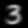
\includegraphics[width=0.11\textwidth]{k_mean_3.png} \ \ \\
            class 0 &  class 1 &  class 2 & class 3\\[3pt]

            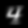
\includegraphics[width=0.11\textwidth]{k_mean_4.png} &
            
\includegraphics[width=0.11\textwidth]{k_mean_5.png} &
            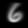
\includegraphics[width=0.11\textwidth]{k_mean_6.png} &
            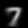
\includegraphics[width=0.11\textwidth]{k_mean_7.png} \\
            class 4 &  class 5 &  class 6  &  class 7\\[3pt]

            & 
\includegraphics[width=0.11\textwidth]{k_mean_8.png} &
              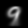
\includegraphics[width=0.11\textwidth]{k_mean_9.png} & \\
            &  class 8 &  class 9 & \\
        \end{tabular}
        \caption{K-means centroids}
        \label{fig:kmeans}
    \end{figure}
\end{center}

The centroids above appear to to be fuzzy. This is because of the variation of images in the same class. It is clearly visible that the
centroids of the class 1 is comprised of ones that lean to the left and ones that lean to the right. This is bad for the classification
as the distance between the centroid and the test images will never be low enough to confidently classify the image.  

The up site of the K-means algorithm is that once the centroids are initialized, the algorithm can classify the images 
in a very efficient way. The centroids can be saved in a file and reused for future classifications. The classification 
process is the same as the KNN algorithm.

\subsubsection{Results}

The K-means algorithm does not perform very well. The reason for this is that digits of the same class can appear in drasticaly different
positions. This means that the centroids could easily be placed in the middle of another class, thus leading to a lot of misclassifications.

The table below shows the accuracy and the execution time of the K-means algorithm. The accuracy is the percentage of the correctly
classified images. The execution time is the time it took to classify all the images in the test dataset. The execution time is measured
in seconds. 16 threads were used for the parallelization of the algorithm.

\renewcommand{\arraystretch}{1.5}

\begin{center}
    \begin{table}[h]
        \centering
        \begin{tabular}{|c|c|c|c|c|}
            \hline
            Run & 1 & 2 & 3 & 4 \\
            \hline
            Accuracy (\%) & 82.06 & 82.06 & 82.06 & 82.06 \\
            \hline
            Time (ms) & 65.8 & 61.16 & 68.42 & 63.55 \\
            \hline
        \end{tabular}
        \caption{K-Means performance}
        \label{tab:kmeans}
    \end{table}
\end{center}

\renewcommand{\arraystretch}{1}


Because the cluster means are initialized from all the data the results of each run are the same. Some misclassifications are shown
in the figure (\ref{fig:kmeans_misclassifications}).

\begin{center}
    \begin{figure}[H]
        \centering
        \begin{tabular}{ccc}
            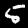
\includegraphics[width=0.15\textwidth]{ncc_misclassified/miss_1_res_2_label_5.png} \ \ &
            
\includegraphics[width=0.15\textwidth]{ncc_misclassified/miss_3_res_7_label_9.png} \ \ &
            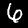
\includegraphics[width=0.15\textwidth]{ncc_misclassified/miss_4_res_4_label_6.png} \ \ \\
            classified as 2 &  classified as 7 &  classified as 4\\[3pt]

        \end{tabular}
        \caption{K-means misclassifications}
        \label{fig:kmeans_misclassifications}
    \end{figure}
\end{center}

The first and second image could easily be misclassified but the third image is a clear misclassification. The image is clearly a 6 but
the algorithm classified it as a 4. The distance between the centroid of the class 4 and the image is 757713 while the distance
between the centroid of the class 6 and the image is 769147. It is a close call but the algorithm should have classified the image.

\subsection{K-means with Advanced Clustering}
\subsubsection{Implementation}

The initialization of the k-means algorithm was performed in a supervised way. The centroids were initialized by iterating over all the
training images and calculating the mean image of each class. This method is not very efficient in two ways. First, the performance of
the algorithm is dependent on the size of the training set. Second the number of classes is fixed. This is a problem because in the MNIST
dataset images from the same class can appear in different positions.

The interpretation of this phenomenon is that images from the same class can have different characteristics, such as size, shape etc.
For example the number 1 can lean to the left or to the right. To combat this problem, the number of clusters are drastically increased.

The initialization algorithm used is the K-means++ algorithm. The K-means++ chooses the first centroid randomly and after that it tries
to choose the next centroids in a way that the distance between the centroids is maximized. The algorithm is described in the paper \cite{kmeans++}.

After the centroids are initialized, training images are assigned to the closest centroid. The class of each centroid is determined by the
most common class of the images assigned to it. The centroids are also updated by calculating the mean image of the images assigned to it.

During the selection and later fitting of the centroids, a random subset of the training images is used. This is done to speed up the 
algorithm but it also prevents the algorithm from overfitting.

The number of the centroids determines the number of distinct features that the algorithm will extract from the images. Below are some selections
of centroids for different number of clusters.

\begin{center}
    \begin{figure}[H]
        \centering
        \begin{tabular}{cccc}
            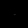
\includegraphics[width=0.15\textwidth]{ncc_centroids/10/mean_cluster_0.png} \ \ &
            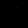
\includegraphics[width=0.15\textwidth]{ncc_centroids/10/mean_cluster_1.png} \ \ &
            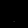
\includegraphics[width=0.15\textwidth]{ncc_centroids/10/mean_cluster_2.png} \ \ &
            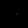
\includegraphics[width=0.15\textwidth]{ncc_centroids/10/mean_cluster_3.png} \ \ \\
        \end{tabular}
        \caption{10 Clusters centroids selection}
        \label{fig:10_clusters}
    \end{figure}
\end{center}

With 10 clusters (\ref{fig:10_clusters}) the centroids average out close to all 0. So the classification is almost random at 20\% accuracy.


\begin{center}
    \begin{figure}[H]
        \centering
        \begin{tabular}{cccc}
            
\includegraphics[width=0.15\textwidth]{ncc_centroids/32/mean_cluster_7.png} \ \ &
            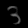
\includegraphics[width=0.15\textwidth]{ncc_centroids/32/mean_cluster_8.png} \ \ &
            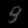
\includegraphics[width=0.15\textwidth]{ncc_centroids/32/mean_cluster_13.png} \ \ &
            
\includegraphics[width=0.15\textwidth]{ncc_centroids/32/mean_cluster_21.png} \ \ \\
        \end{tabular}
        \caption{32 Clusters centroids selection}
        \label{fig:32_clusters}
    \end{figure}
\end{center}

With 32 clusters (\ref{fig:32_clusters}) the centroids are more distinct. The first image is an 8, the second is probably a 3, the third is a 9 and
the fourth is a 5. The accuracy is close to 60\%.

\begin{center}
    \begin{figure}[H]
        \centering
        \begin{tabular}{cccc}
            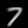
\includegraphics[width=0.15\textwidth]{ncc_centroids/128/mean_cluster_4.png} \ \ &
            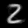
\includegraphics[width=0.15\textwidth]{ncc_centroids/128/mean_cluster_5.png} \ \ &
            
\includegraphics[width=0.15\textwidth]{ncc_centroids/128/mean_cluster_17.png} \ \ &
            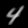
\includegraphics[width=0.15\textwidth]{ncc_centroids/128/mean_cluster_20.png} \ \ \\
        \end{tabular}
        \caption{128 Clusters centroids selection}
        \label{fig:128_clusters}
    \end{figure}
\end{center}

With 128 clusters (\ref{fig:128_clusters}) the centroids are even more distinct. There are some problems with specific numbers such as 3 and 8. For 
example the 3rd image could be a 3 or a 8. The accuracy is close to 80\%.

\begin{center}
    \begin{figure}[H]
        \centering
        \begin{tabular}{cccc}
            
\includegraphics[width=0.15\textwidth]{ncc_centroids/350/mean_cluster_7.png} \ \ &
            
\includegraphics[width=0.15\textwidth]{ncc_centroids/350/mean_cluster_24.png} \ \ &
            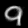
\includegraphics[width=0.15\textwidth]{ncc_centroids/350/mean_cluster_28.png} \ \ &
            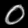
\includegraphics[width=0.15\textwidth]{ncc_centroids/350/mean_cluster_29.png} \ \ \\
        \end{tabular}
        \caption{350 Clusters centroids selection}
        \label{fig:350_clusters}
    \end{figure}
\end{center}

Finally with 350 clusters (\ref{fig:350_clusters}) the centroids are very distinct. The accuracy is close to 90\%. This number of clusters produces
the best results.

For all the tests the number of iteration during fitting was set to 30, as this was the number that produced the best results.

\subsubsection{Results}

\renewcommand{\arraystretch}{1.5}

\begin{center}
    \begin{table}[h]
        \centering
        \begin{tabular}{|c|c|c|c|c|}
            \hline
            Number of clusters & 10 & 32 & 128 & 350 \\
            \hline
            Accuracy (\%) & 15.99 & 53.53 & 86.58 & 91.38 \\
            \hline
            Cluster Creation Time (s) & 3.1 & 7.38 & 26.35 & 77.18 \\
            \hline
            Image Classification Time (s) & 0.061 & 0.175 & 0.677 & 2.034 \\
            \hline
        \end{tabular}
        \caption{K-Means++ clustering performance}
        \label{tab:clustering}
    \end{table}
\end{center}

\renewcommand{\arraystretch}{1}

The increasing cluster creation time is not a problem as it is done only once. The produces centroids can be saved and used for future classification.